\classDate{Mo.\\03/12/18}
\subsection{Continuous time infinite horizon DP}

\begin{optExample}{Problem setup}
\begin{align*}
    \min \intdt{0}{t_f = \infty}{ f_0 \paren{x,u} }
\end{align*}
\begin{align*}
    \txt{s.t.} \quad \dot{x} &= f\paren{x,u}\\
    u(t) &\in \setU{x\paren{t}}
\end{align*}
\end{optExample}

\paragraph{Assumptions}
\begin{itemize}
    \item $f_0 \paren{x,u} \geq 0 \quad \forall ~ x,u, \quad x \in \R^n, u \in \R^q$
    \item $f_0 \paren{x,u} > 0$ whenever $u\neq 0$
    \item $f_0 \paren{x,0}$ is zero state detectable\\
        i.e., $y = f_0 \paren{x\paren{t},0} \rightarrow 0 \Rightarrow x(t) = 0$
    \item $f_0 \paren{0,0} = 0$
\end{itemize}

\paragraph{Cost-to-go} $J \paren{x_1,t_1}$\\
``Cost with $x_1$ as new initial condition.''
\begin{align*}
J \paren{x_1,t_1} = \min_{u} \intdt{t_1}{\infty}{f_0 \paren{x,u}}
\end{align*}

\subparagraph{$t_f < \infty$}
\begin{align*}
    -\pdein{J \paren{t,x}}{t} &= \minux{} \set{f_0 \paren{x,u} + \pdein{J \paren{t,x}}{x}f \paren{x,u} }
\end{align*}

\subparagraph{$t_f = \infty$}
\begin{align*}
\txt{cost-to-go } &\corresponds \txt{ cost/value function}\\
J \paren{t_1,x_1} &= V \paren{x_1}\\
    0 &= \minux{} \set{f_0 \paren{x,u} + \pdein{V \paren{x}}{x}f \paren{x,u} }
\end{align*}

\paragraph{Main questions}
\begin{enumerate}
\renewcommand{\labelenumi}{\alph{enumi})}
\item Optimality, stability
\item Robustness
\end{enumerate}

\paragraph{a) Optimality, stability} ~\\
\begin{theorem}{}
Suppose the assumptions above hold true.
Let $\Vbar{} \in C^1$, which is positive definite
\bluetext{and radially unbounded}, be
\def\funcVal{f_0 \paren{x,u} + \pdein{\Vbar{x}}{x} f \paren{x,u}}
    \begin{align*}
    \txt{s.t.} \quad
    0 &= \minux{} \set{\funcVal}\\
    \txt{and } \ubar{x} &= \argmin \set{\funcVal}
    \end{align*}
then $\Vbar{} = V$ (value function $V^*$) and $\ubar{}$ is an optimal feedback which is \bluetext{globally} asymptotically stabilising (w.r.t. $x=0$).
\end{theorem}

\paragraph{Proof} ~\\
Step 1: stability
\begin{align*}
0 &= f_0 \paren{x, \ubar{x}} + 
    \underbrace{\pdein{\Vbar{x}}{x} f \paren{x,\ubar{x}}}
    _{\Vbard{x} = L_f\Vbar{x}}
\quad \txt{HJBE}\\
\Vbard{x} &= -f_0 \paren{x,\ubar{x}} \leq 0\\
\Rightarrow x &= 0 \txt{ is \bluetext{globally} stable}
\end{align*}
Provided $\Vbar{}$ is positive definite \bluetext{and radially unbounded}.\\

Step 2: asymptotic stability
\begin{align*}
\Vbard{x} = -f_0 \paren{x,\ubar{x}}
\end{align*}
\begin{gather*}
\txt{(La Salle)} \quad x(t) \rightarrow \set{x: \Vbard{x} = 0 = f_0 \paren{x,\ubar{x}}=0}
\intertext{Fox $f_0 \paren{x,u} > 0, u\neq 0$:}
\Rightarrow x(t) \rightarrow \set{x: f_0 \paren{x,0} = 0}
\end{gather*}

Step 3: HJBE
\begin{gather*}
0 \leq f_0 \paren{x,u} +
    \underbrace{\pdein{\Vbar{x}}{x} f \paren{x,u}}_{\Vbard{}}
    \quad \forall ~u(x)\in \setU{x}\\
\left( 0 = f_0 \paren{x,u} +
    \pdein{\Vbar{x}}{x} f \paren{x,u} \right)
\end{gather*}
\begin{align*}
\-\Vbard{x} &\leq f_0 \paren{x,u}\\
\Vbar{x_0} - \Vbar{x(t)} &\leq \int_0^t f_0 \paren{x,u} d\tau, \quad t \rightarrow \infty\\
\Vbar{x_0} &\leq \int_0^\infty f_0 \paren{x,u} d\tau \quad \forall    ~ u(x) \in \setU{x}, \txt{n}\footnotemark
\end{align*}
\footnotetext{in particular $u^* \in \setU{x}$}

\begin{itemize}
\item $\Vbar{x_0}$ is a lower bound of the value function ($\Vbar{} \leq V$)
\item $\Vbar{}$ is achieved by $\ubar{}$, hence $\Vbar{} = V, \ubar{} = u^*$
\end{itemize}

\paragraph{b) Robustness}~\\
Setup:
\begin{gather*}
\min \intdt{0}{\infty}{q(x) + u^R(x)u} \quad u \in \R^q, x\in\R^n\\
\txt{s.t. } \dot{x} = f(x) + G(x)u, \quad q(x)>0, R(x)>0
\end{gather*}

HJBE:
\begin{align*}
    \begin{split}
        0 &= \min \left\lbrace q(x) + u^T R(x)u \right. \\
            &\quad \left. + \pdein{\Vbar{x}}{x}f(x) + \pdein{\Vbar{x}}{x}G(x)u \right\rbrace
    \end{split} \numberthis \label{eq:hjbe-robustness}
\\
\pde{u}\set{.} &= 2R(x)\ubar{} + G^T(x)\pdein{\Vbar{}^T(x)}{x} = 0\\
\ubar{x} &= -\frac{1}{2} \inv{R}(x) G^T(x) \pdein{\Vbar{}^T(x)}{x}
\numberthis \label{eq:hjbe-robustness-ubar}\\
\ubar{x} &= -\frac{1}{2} \inv{R}(x) L_g V \paren{x}, \quad u \in \R, \paren{G = \varphi}
\end{align*}
"$L_gV$" control law $\rightarrow$ nonlinear control
\begin{align*}
\intertext{Substitute \eqn{eq:hjbe-robustness-ubar} in \eqn{eq:hjbe-robustness}}
    \begin{split}
        0 &= q(x) + \frac{1}{4} \pdein{V \paren{x}}{x}G(x)R(x) G^T(x)\pdein{V^T(x)}{x}\\
            &\quad + \pdein{V(x)}{x}f(x) - \frac{1}{2}\pdein{V(x)}{x}G(x)\inv{R}(x)G^T(x)\pdein{V^T(x)}{x}
    \end{split}\\
    \begin{split}
        0 &= q(x) -\frac{1}{4}\pdein{V(x)}{x}G(x)\inv{R}(x)G^T(x)\pdein{V^T(x)}{x}\\
            &\quad + \pdein{V(x)}{x}f(x)
    \end{split}\\
0 &= q(x) + \frac{1}{2}\pdein{V(x)}{x}G(x)\ubar{x} + \pdein{V(x)}{x}f(x)
\end{align*}

\paragraph{Uncertainties} e.g. actuator nonlinearities (unmodelled)
\begin{figure}[H]
    \centering
    \tikzsetnextfilename{uncertainties}
    \begin{tikzpicture}[every node/.append style={font=\footnotesize}]
    \def\w{3cm}
    \node (sys) [block,text width=\w] {$\dot{x} = f(x) + G(x)u$};
    \node (del) [block,text width=0.22*\w,left=0.3*\w of sys] {$\Delta(\ubar{})$};
    \node [above=1mm of del.north] {input uncertainty};
    \node [left=0.15*\w of del.west,inner sep=0mm] (dell) {};
    \node (ubr) [block,text width=0.22*\w,below=0.22*\w of sys] {$\ubar{x}$};
   
    \begin{scope}[arrow]
    \draw (sys.east) -- ++(0.15*\w,0) |- (ubr);
    \draw (ubr) -| (dell) -- (del);
    \draw (del) -- (sys);
    \end{scope}
    \end{tikzpicture}
\end{figure}

For which $\Delta$'s is the closed-loop asymptotically stable?
\def\starlVal{
    \pdein{V(x)}{x}G(x)
    }
\def\starrVal{
    \paren{\Delta\paren{\ubar{}} - \frac{1}{2}\ubar{x}}
    }
\begin{align*}
    (\Vbard{} = ) \dot{V}(x) &= \pdein{V(x)}{x}\paren{f(x) + G(x\Delta\paren{\ubar{}}}
        \overset{!}{\leq} 0\\
    \dot{V}(x) &= \pdein{V(x)}{x}f(x) + \frac{1}{2}\pdein{V(x)}{x}G(x)\ubar{x}\\
        &\quad - \frac{1}{2}\pdein{V(x)}{x}G(x)\ubar{x}
        + \pdein{V(x)}{x}G(x)\Delta\paren{\ubar{}}\\
        &= \underbrace{-q(x)}_{<0} + \underbrace{\starlVal\starrVal}_{*}
\end{align*}%

Asymptotically stable if $* \leq 0$:
\begin{align*}
    \underbrace{\starlVal}_{-2\ubar{}^TR}
        \starrVal &\leq 0\\
    -2\ubar{}^T(x)R(x)\starrVal{}
        & \overset{?}{\leq} 0\\
    \ubar{}^T(x)R(x)\starrVal{}
        & \overset{?}{\geq} 0\\
\end{align*}

\paragraph{q=1} $( u \in \R ) \quad R(x) = r(x) > 0$
\begin{align*}
    \ubar{} \cdot \starrVal{} &\geq 0\\
    \ubar{} \Delta\paren{\ubar{}} - \frac{1}{2}\ubar{}^2 &\geq 0\\
\end{align*}%
\begin{figure}[H]
    \centering
    \def\svgwidth{0.7\columnwidth}
    \input{./img/ubar-uncertainty.pdf_tex}
\end{figure}

Remark:
\begin{figure}[H]
    \centering
    \def\svgwidth{0.7\columnwidth}
    \input{./img/ubar-uncertainty-sector.pdf_tex}
\end{figure}

\paragraph{$q>1$}~\\
\begin{theorem}{{(similar to $q=1$)}}
Suppose
\begin{align}
R(x) &= \matr{r_x(1) & & 0\\
            & \ddots \\
        0 & & r_q(x)}\\
\Delta(\ubar{}) &= \matr{
    \Delta_1(\ubar{}_1\\
    \vdots\\
    \Delta_q(\ubar{}_q
    }
\end{align}
then $\ubar{}$ achieves a sector margin of $[1/2, \infty]$
\end{theorem}

Remark:
\begin{itemize}
    \item LQR gain margin $[1/2, \infty]$
    \item disc margin (as a generalisation of phase margin)\\
    $\rightarrow$ nonlinear control
\end{itemize}
\begin{figure}[H]
    \centering
    \tikzsetnextfilename{nonlin-ctrl}
    \begin{tikzpicture}[every node/.append style={font=\footnotesize}]
    \def\w{3cm}
    \node (sys) [block,text width=0.8*\w] {$\dot{x} = f(x) + G(x)u$};
    \node (comp) [comp,left=0.14*\w of sys.west] {};
    \node (in) [left=0.2*\w of comp] {$v$};
    \node (ubr) [block,text width=0.22*\w,below=0.18*\w of sys] {$\ubar{x}$};
    \node (cout) [cout,right=0.1*\w of sys.east] {};
    \node (out) [block,right=0.2*\w of cout,text width=0.525*\w,inner sep=1mm] {$y=-\ubar{x}$};
    
    \begin{scope}[arrow]
    \draw (sys.east) -- (cout) |- (ubr);
    \draw (ubr) -| (comp.south) node [left,pos=0.9] {+};
    \draw (comp) -- (sys);
    \draw (in) -- (comp) node [above,pos=0.9] {+};
    \draw (cout) -- (out);
    \draw (out.east) -- ++(0.14*\w,0) node [above] {$y$};
    \end{scope}
    \end{tikzpicture}
\end{figure}

From $v \rightarrow y$, system is passive, i.e.
\begin{align*}
    \dot{V} = -\frac{1}{2}y^Ty + y^Tv
\end{align*}
Passive systems
\begin{figure}[H]
    \centering
    \tikzsetnextfilename{passive-sys}
    \begin{tikzpicture}[every node/.append style={font=\footnotesize}]
    \def\w{3cm}
    \node (sys) [block,text width=0.8*\w] {passive};
    \node (comp) [comp,left=0.2*\w of sys.west] {};
    \node (ubr) [block,text width=0.8*\w,below=0.18*\w of sys] {passive};
    
    \begin{scope}[arrow]
    \draw (sys.east) -- ++(0.2*\w,0) |- (ubr);
    \draw (ubr) -| (comp.south) node [left,pos=0.9] {-};
    \draw (comp) -- (sys);
    \end{scope}
    \end{tikzpicture}\\
    $\Rightarrow$ `` overall system is passive''
\end{figure}

\paragraph{Example}
\begin{align*}
    \dot{x} &= x^2 + u\\
    u &= -x^2 - x \Rightarrow \txt{ closed loop}\\
    \Rightarrow \dot{x} &= -x \quad \txt{ FB linearisation}
\end{align*}
\begin{align*}
    \Delta(u) &= \paren{1 + \varepsilon} u, \quad \varepsilon > 0\\
    \dot{x} &= x^2 + \paren{1 + \varepsilon} \paren{-x^2 -x}\\
        & -\paren{1 + \varepsilon}x - \varepsilon x^2
\end{align*}
$\rightarrow$ closed loop is not globally stable -- even worse,
shows finite escape behaviour%
\footnote{finite escape behaviour $\corresponds \modl{x(t)} \rightarrow \infty, t \rightarrow t^*$, ``system explodes'' },
even for small uncertainties.

\paragraph{Integrating the HJBE:}
\begin{align*}
    V(x) &= \frac{2}{3}x^3 + \frac{2}{3}\paren{1+x^2}^{\frac{3}{2}} - \frac{2}{3} > 0
    \quad \txt{pos. def.}
\end{align*}
\begin{figure}[H]
    \centering
    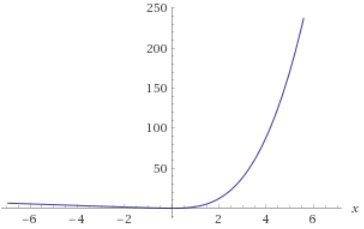
\includegraphics[width=0.8\columnwidth]{img/vx-posdef.png}
\end{figure}
\begin{align*}
    \min & \intdt{0}{\infty}{\underbrace{x^2 + u^2}_{f_0}}\\
    \ubar{x} &= -x^2 - \underbrace{\paren{\sqrt{1 + x^2}}}_{\txt{state-dependent gain}} x
\end{align*}

\paragraph{Remark}
\begin{itemize}
    \item \textbf{Inherent robustness}\\
            uncertainties/unmodelled dynamics are not taken into account in the control design
    \item \textbf{Robust design}\\
            uncertainties are explicitly taken into account in the control design\\
            worst case represented by maximum disturbance $w$
            (unmodelled dynamics) $\rightarrow \max_w$
\begin{align*}
    \min_u \max_w &\intdt{0}{\infty}{f_0 \paren{x,u,w}}\\
    \txt{s.t. } &\quad \dot{x} = f \paren{x,u,w}
\end{align*}
HJBIE\footnote{I: Isaacs}:
\begin{align*}
    0 &= \min_u \max_w \set{f_0 + \Vbard{}}
\end{align*}
(2 player zero sum differential game)
    \begin{itemize}
        \item $u$: control engineer
        \item $w$: nature/disturbance
    \end{itemize}
    $\rightarrow$ LQ-Setup: $H_2/H_\infty$ control (robust control)
    \item \textbf{Inverse optimality}\\
        ``normal case'': use value function as Lyapunov function\\
        ``inv. opt'': use control/Lyapunov function as value function\\
        \\
        Applications: robust stabilisation, nonlinear control
\end{itemize}
